\documentclass{article}

\begin{document}

\title{Adventures in (informatically simulated) recreational mathematics: An introduction to big-O notation, and these plural heresies with which to conduct multiplication with increasingly full vigour}
\date{4 September 2017}
\author{Benedict Randall Shaw}

\maketitle

DISCLAIMER: this edition of ARM contains neither traditional maths nor any pretty pictures; rather, we are stepping out into the related field of computer science, and are stuck with graphs. We apologise for any inconvenience caused.

\section{Big-O Notation}

In computer science, one seeks to write efficient algorithms, so as not to waste valuable processing time. However, as counterintuitive as it sounds, what we care about most is not how well a program performs on a given value, but rather how well it scales to more complex situations.\\

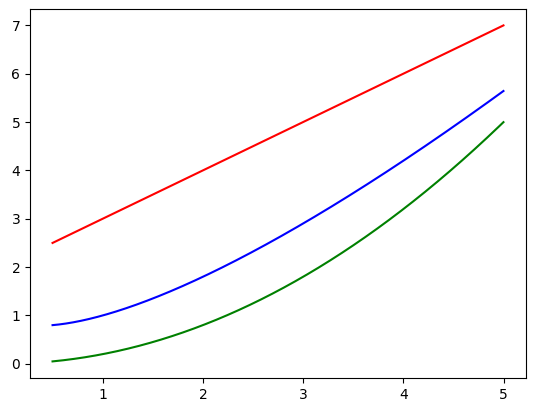
\includegraphics{smallgraph}

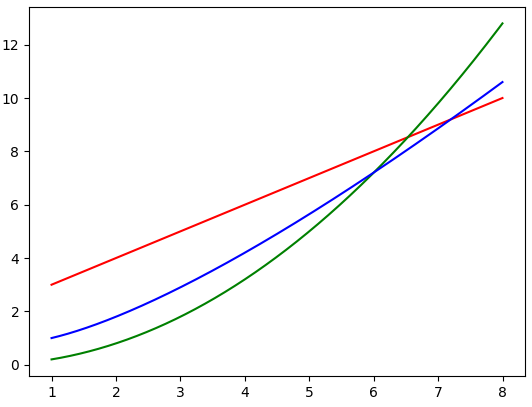
\includegraphics{mediumgraph}

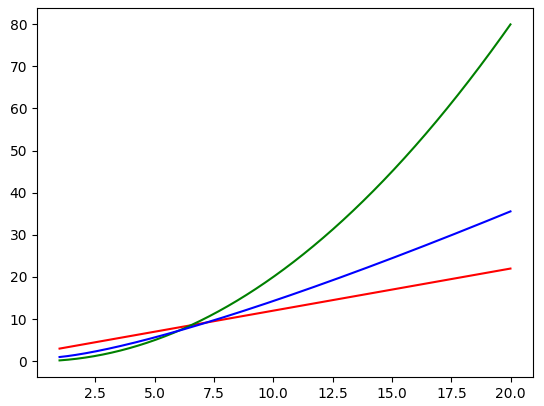
\includegraphics{largegraph}

Consider three programs which sort a list of length \(n\), which we'll call the red, blue, and green programs. We now graph the worst-case (longest) period of time required for each of these programs against the lengths of list, shown at different scales in Figures 1, 2, and 3. From Figure 1, it would seem that the green program is the quickest; however, for most values it turns out to be by far the worst. We don't usually care about comparing the time taken to sort short lists, as this can be done very quickly either way, and the differences in time taken aren't actually that large. What we care about are cases where the list is long, as shown on the far right of Figure 3, as the slowest programs can take many times to longer to run than the fastest. In fact, in many such problems, even algorithms which both look at the small scale to be similar (e.g. the blue and green programs) grow to be have very different performances eventually. Computer scientists describe the rate of growth of running times using \textit{big-O notation}.

We say that \(f(n)=O(g(n))\), where \(f\) and \(g\) are functions on the real numbers, if there exist positive real numbers \(M\) and \(y\) such that for all values of \(n \geq{} y\), \(|f(n)|\leq{}|Mg(n)|\). At face value, it may seem that by making \(M\) very large, any program must take less than \(Mg(n)\) units of time to run. This is not the case, as can be illustrated with \(f(n)=n^2\) and \(g(n)=n\); for any value of \(M\), for all values of \(n>M\), \(f(n)=n^2>Mn=Mg(n)\) as \(n>M\), so \(f(n)>Mg(n)\) eventually for all values of \(M\). What we really mean in a nutshell by \(f(n)=O(g(n))\) is that \(f(n)\) doesn't grow more quickly than \(g(n)\)\footnote{This phrasing is a slight oversimplification, but helpful to consider in order to understand the concept.}. There are a variety of other pieces of big-O notation. For example, we say \(f(n)=\Omega(g(n))\) if there exist positive real numbers \(N\) and \(z\) such that for all values of \(n \geq{} z\), \(|f(n)|\geq{}|Ng(n)|\); this essentially means that \(f(n)\) doesn't grow less quickly than \(g(n)\)\footnotemark[\value{footnote}]. We also say that \(f(n)=\Theta(g(n))\) if \(f(n)=O(g(n))\) and \(f(n)=\Omega(g(n))\) (that is to say, if \(f(n)\) grows roughly as quickly as \(g(n)\)\footnotemark[\value{footnote}]).

Interestingly, if a function \(f(n)=g(n)+h(n)\), and \(g(n)\) grows at least as quickly as \(h(n)\), and \(g(n)=O(d(n))\) for some function \(d\), then as past a certain point \(g(n)\geq{}h(n)\), and past said point \(f(n)\leq{}2g(n)\leq2Md(n)\), so \(f(n)=O(d(n))\) too (as \(f(n)\leq{}2Md(n)\) and \(2M\) is a constant real number). What this really means is that a function grows as quickly as its fastest growing term; for example, if \(f(n)=2x^3 + 5n^2 + 2\log(n) + 11\), then \(f(n)=O(x^3)\) as \(2x^3\) grows more quickly than the other terms. For this, it is helpful to have some idea about which functions grow more quickly than others; a chart of such functions is given at the end of this section.

In computer science, we care predominantly about the worst-case running time; it (usually) causes no problems if a program runs quickly, but a program taking ages to run is to be avoided if the program is to be usable. We therefore tend to prioritise \(O\) over \(\Omega\) and \(\Theta\). We say a program has \textit{time complexity} of \(O(g(n))\) (or sometimes we just say that it is \(O(g(n))\)) if its worst case running time in arbitrary time units is \(O(g(n))\); for example, the red program in Figures 1--3 is linear and so has time complexity \(O(n)\). (It is also technically \(O(n^2)\), as \(n^2\) grows faster than a linear function, but this is unhelpful, so the time complexity uses the slowest growing function we can possibly place inside the brackets of \(O()\).) We have names for some time complexities; for example, we say the red program has linear time complexity, for obvious reasons. Below is a chart of common time complexities and their names, ordered from slowest to fastest growing.

\begin{center}
	\begin{tabular}{c|c}
		\(O(1)\)&constant\\\hline
		\(O(\log*n))\)&log-star\footnotemark\\\hline
		\(O(\log(\log{}n))\)&double logarithmic\\\hline
		\(O(\log{}n)\)&logarithmic\\\hline
		\(O(n^c)\) where \(0<c<1\) is a constant&fractional power\\\hline
		\(O(n)\)&linear\\\hline
		\(O(n\log{}n)\)&linearithmic\\\hline
		\(O(n^c)\) where \(1<c<2\) is a constant&polynomial\\\hline
		\(O(n^2)\)&quadratic (also polynomial)\\\hline
		\(O(n^c)\) where \(2<c<3\) is a constant&polynomial\\\hline
		\(O(n^3)\)&cubic (also polynomial)\\\hline
		\(O(n^c)\) where \(3<c\) is a constant&polynomial\\\hline
		\(O(c^n)\) where \(1<c\) is a constant&exponential\\\hline
		\(O(n!)\)&factorial
	\end{tabular}
\end{center}
\footnotetext{\(\log*n\) is the number of times the logarithm function must be iteratively applied to \(n\) before \(n\leq{}1\).}

\section{Long multiplication}

It is necessary for a computer to be able to carry out arithmetic operations as quickly as possible, as these are the building blocks of most programs. We can add two \(n\)-bit\footnote{binary digit} numbers (those less than \(2^n\)) with \(O(n)\) time complexity on a sequential circuit through the usual method that one is taught in school; one simply goes through the two numbers bit by bit, starting with the least significant, and adds them, carrying over into the next column if one needs to. One must only ever add a maximum of three bits (two from the numbers and one from carrying) each time, each individual bit addition has constant time complexity. Because one goes through \(n\) such sets of bits, addition has \(O(n)\) time complexity.

Multiplication is trickier. However, in the same way that we find it very easy to multiply by powers of 10 by adding zeroes, modern computers are able to multiply by powers of two with \(O(1)\) time complexity (using a circuit called a barrel shifter which will not be explained here). This is called a bit shift, and is very helpful. It means that the long multiplication algorithm, which probably we have all used at some point or other, can be done fairly quickly on a computer. For two \(n\)-bit numbers, long multiplication gives us an intermediate term for each ``1'' bit of the first of the numbers to be multiplied. In the worst case scenario, there are \(n\) of these terms, and as each is produced in constant time from bit shifts, the production of these has \(O(n)\) time complexity.

As they are all the product of an \(n\)-bit number and a power of two that fits in \(n\)-bits, the terms fit in \(2n\) bits. Thus we are adding \(n\) \(2n\)-bit numbers, so we must perform \(n-1\) addition operations. As addition is \(O(n)\), this means that the summation of the intermediate terms has \((n-1)\times{}O(2n)=O(2n^2-2n)=O(n^2)\) time complexity. The production of the terms is \(O(n)\), so the time complexity of long multiplication is \(O(n)+O(n^2)=O(n^2)\). This is pretty bad. If we wanted to multiply two ten-million-digit numbers (33 million bits), and we were able to perform a billion single-bit additions a second, this algorithm would take nearly a fortnight.

\section{Karatsuba's algorithm}

It was conjectured by Andrey Kolmogorov, a notable Soviet mathematician, that the quadratic time complexity of long multiplication could not be improved upon. In 1960, he held a seminar at which he mentioned this, among other computational complexity problems. A week later, Anatoly Karatsuba, a 23-year-old student, found this algorithm, which runs with \(O(n^{log_{2}3})\approx{}O(n^{1.585})\) time complexity.

It belongs to a class of algorithms known as ``divide and conquer'' algorithms. These work by splitting problems into smaller instances of the same type of problem, until they can be solved easily, and then recombining the solutions to solve the initial problem.

Consider multiplying two \(n\)-bit integers, \(x\) and \(y\). Let \(m\) be \(\left\lceil\frac{n}{2}\right\rceil\). Then by splitting \(x\) and \(y\) down the middle, we can obtain \(x_1,x_0,y_1,y_0<2^m\) such that \(2^{m}x_1+x_0=x\)\(2^{m}y_1+y_0=y\)

Then it follows that \(xy=2^{2m}x_1y_1+2^m(x_1y_0+x_0y_1)+x_0y_0\)

There are 4 multiplications to be performed here, and one method of multiplication has you do them all individually; then one does those multiplications by the same technique, and so on until the multiplications are all single-bit, upon which you do them by the usual method. Suppose it takes \(T(n)\) basic operations (single-bit additions and multiplications) to multiply two \(n\)-bit numbers by this method; then this method gives \(T(n)=4T(\left\lceil{}\frac{n}{2}\right\rceil{})+6n\), as we have to add 4 \(2n\)-bit numbers, which require 3 additions (so require \(6n\) basic operations in total).

This is called a recurrence relation, and can be solved by through a variety of means. For the sake of brevity, we shall use the master theorem, which tells us that, where \(T(n)=aT(\frac{n}{b})+f(n)\), and \(c_{crit}=\log_ba\) (the \textit{critical exponent}): when \(f(n)=O(n^c\) for some \(c<c_{crit}\) (i.e. the work to split and recombine a problem is far less than that of the subproblems), \(T(n)=\Theta(n^{c_{crit}})\); when \(f(n)=\Theta(n^{c_{crit}}log^kn)\) for some \(k\geq0\) (i.e. the work to split and recombine a problem is comparable to that of the subproblems), \(T(n)=\Theta(n^{c_{crit}}log^{k+1}n)\); and when \(f(n)=\Omega(n^c)\) for some \(c>c_{crit}\) (i.e. the work to split and recombine a problem is far greater than that of the subproblems), \(T(n)=\Theta(f(n))\).

In the case of the algorithm we are currently considering, \(T(n)=4T(\frac{n}{2})+6n\) (we have dropped the ceiling signs, as they make a tiny change in the grand scheme of things to \(\frac{n}{2}\) which does not affect the time taken significantly). Thus \(c_{crit}=\log_{2}4=2\) and \(f(n)=6n=O(n^1)\) so \(c=1<c_{crit}\). The master theorem then tells us that \(T(n)=\Theta(n^2)\), which is no better than long multiplication.

What Karatsuba hit upon was that \(xy=2^{2m}x_1y_1+2^m(x_1y_0+x_0y_1)+x_0y_0\) could be calculated with only 3 subproblems. We calculate \(z_2=x_1y_1\) and \(z_0=x_0y_0\). Then we calculate \(z_1=(x_1+x_0)(y_1+y_0)-z_2-z_0\), which is equal to \(x_1y_0+x_0y_1\). Thus we have only made three multiplications, and a couple of additions and subtractions, both of which have linear time complexity. Thus Karatsuba's algorithm gives us \(T(n)=3T(n/2)+f(n)\), where \(f(n)=O(n)\). By the master theorem, \(c_{crit}=\log_{2}3\), so as \(f(n)=O(n^1)\), \(c<c_{crit}\), and \(T(n)=\Theta(n^{\log_{2}3})\approx{}\Theta(n^{1.585})\).

This means that in our previous example of two ten-million-digit numbers, we would be done in a couple of hours. This is a marked improvement, but we can still do better.

\section{Toom-Cook}

In 1963, Andrei Toom described a generalisation of the Karatsuba algorithm, which Stephen Cook improved as his PhD in 1966. It uses the technique of splitting numbers up (as in Karatsuba) and treating them as polynomials, which is also used in the Sch\"onhage-Strassen algorithm, which is faster still.

Long multiplication is Toom-1, and has time complexity \(=O(n^2)\). The Karatsuba algorithm is Toom-2, and has time complexity \(\approx{}O(n^1.585)\). Toom-3 has time complexity \(\approx{}O(n^1.465)\). In general, Toom-\(k\) has time complexity \(\Theta(c(k)n^{log(2k-1)/log(k)})\), where \(c(k)\) is the time spent on addition and multiplication by small constants. Unfortunately, the function \(c(k)\) grows very quickly. Through use of a variety of values of \(k\), Donald Knuth has made a Toom-Cook implementation that runs in \(\Theta(n2^{\sqrt{2\log{}n}}\log{}n)\) Due to overhead, Toom-Cook is slower than long multiplication for small numbers. We shall consider Toom-3 as an example; however, we shall give the general algorithm of Toom-\(k\) for any value of \(k\).

Given \(n\)-digit numbers \(x\) and \(y\) (we'll use \(31415926\) and \(2718281\)), we start by splitting each into \(k\) digits in some base \(B=b^i\) for some integer \(i\), where we have the numbers in base \(b\).

Let these \(k\) digits of \(x\) be the coefficients of a polynomial \(P\), and those of \(y\) be coefficients of a polynomial \(Q\). These polynomials have degree \(k-1\). Then \(Q(B)=x\) and \(Q(B)=y\). Call the coefficients of \(P\) \(x_2\), \(x_1\), \(x_0\), such that \(x_i\) is the coefficient of \(n^i\). Similarly, call the coefficients of \(Q\) \(y_2\), \(y_1\), \(y_0\). If we let \(B=1000\) in our example:

{\(P(n)=31n^2+415n+926 \implies P(B)=31415926=x\)}

\(Q(n)=2n^2+718n+281 \implies Q(B)=2718281=y\)

We then want to find the product polynomial \(R(n)=P(n)Q(n)\), which will be of the form \(R(n)=z_4n^4+z_3n^3+z_2n^2+z_1n+z_0\), as we will then be able to easily evaluate \(R(B)=P(B)Q(B)=xy\), as the terms will be easy to calculate using the bit shift mentioned in the section on long multiplication. We do this by interpolation; we find \(2k-1\) values of \(R(n)\), and work out the coefficients from that. Where the values of \(n\) are small, the values of \(P(n)\) and \(Q(n)\) are easy to calculate. We abuse notation by saying that \(P(\infty)\) is the value of the highest-degree coefficient of \(P\). For Toom-3, we shall therefore use \(-1\), 0, 1, 2, and \(\infty\).

\(R(-1)=z_4-z_3+z_2-z_1+z_0\)

\(R(0)=z_0\)

\(R(1)=z_4+z_3+z_2+z_1+z_0\)

\(R(2)=16z_4+8z_3+4z_2+2z_1+z_0\)

\(R(\infty)=z_4\)

We can calculate all of these values by multiplying \(P(n)\) and \(Q(n)\); this uses five multiplications of numbers of length \(\frac{n}{3}\). The coefficients of \(R\) can be figured out from the five values of \(R(n)\) with simple algebra thus:

\(R(\infty)=z_4\)

\(R(0)=z_0\)

\(R(1)+R(-1)=2z_4+2z_2+2z_0\)

\(\frac{R(1)+R(-1)}{2}=z_4+z_2+z_0\)

\(\frac{R(1)+R(-1)}{2}-z_4-z_0=z_2\)

\(R(1)-R(-1)=2z_3+2z_1\)

\(R(2)-16z_4-4z_2-z_0=8z_3+2z_1\)

\(R(2)-16z_4-4z_2-z_0-(R(1)-R(-1))=6z_3\)

\(\frac{R(2)-16z_4-4z_2-z_0-(R(1)-R(-1))}{6}=z_3\)

\(\frac{R(1)-R(-1)}{2}=z_3+z_1\)

\(\frac{R(1)-R(-1)}{2}-z_3=z_1\)

From this we have found the coefficients of \(R\); we can now easily use bit shifts to evaluate \(R(B)=P(B)Q(B)=xy\). Thus we have only used 5 multiplications of length \(\frac{n}{3}\) to calculate a multiplication of length \(n\), with some linear time complexity calculations in between. This means that by the master theorem from earlier, Toom-3 is \(O(n^{log_{3}5})\).

\section{Faster algorithms}

In 1971, Arnold Sch\"onhage and Volker Strassen created the Sch\"onhage-Strassen algorithm, which has time complexity \(O(n\log{}n\log(\log{}n))\). It is faster than Toom-Cook for integers greater than \(2^{2^17}\), that is to say, those with 40,000 decimal digits. It essentially splits the numbers into digits in some base, takes the discrete Fourier transform or them, multiplies the remaining vectors element by element, and then takes the inverse discrete Fourier transform, and conducts carrying.

The F\"urer algorithm was discovered in 2007; it has time complexity \(O(2^{O(\log*n)}n\log{}n)\), and is better than Schönhage-Strassen for integers above \(2^{2^{64}}\). An implementation was made in 2015 with running time \(O(2^{3\log*n}n\log{}n)\), thus removing the nested big-O notation.

\section{Problems}

\begin{enumerate}
	\item Design a sorting algorithm and work out its time complexity. Try to find the most efficient one you can!
	\item Arnold Sch\"onhage and Volker Strassen conjecture that the lower bound of time complexity for multiplication is \(\Omega(n\log{}n)\). Prove this.
\end{enumerate}

\end{document}
